In order to gain a deeper understanding of the testability of the commit history of software projects, we will conduct a case study, which is aimed to be an exploratory research with quantitative data analysis. 
In this case study, we will make an exploratory analysis of different projects, checking if the proposed testability metric (\textit{FullyTestability}) is able to represent the reality of the testability of the projects in all their history.
To quantitatively analyze the projects, we will use a graph per project that represents the results per commit of the steps described in the methodology. 

As can be seen in Figure~\ref{fig:projects-1}, each sub-figure represents the commit history of a project, where the X axis shows the commit number (0 for the first commit of the project, 1 for the second, etc.). On the Y axis we observe a stacked bar for each commit, with the height being the number of tests executed in that commit and the colors (red, orange and green) indicating the results of each test (failure, error and success respectively. Additionally, the graph includes for each commit on the X-axis the number of lines of code (in blue) and test code (in purple), being necessary to look at the values on the right Y-axis.

%%%%%%%%%%%%%%%%%%%%%%%%%%%%%%%%%%%%%%%%%%%%%%%%%%%%%%%%%%%%%%%%%%%%%
%                            FIRST SET                              %
%%%%%%%%%%%%%%%%%%%%%%%%%%%%%%%%%%%%%%%%%%%%%%%%%%%%%%%%%%%%%%%%%%%%%

The first set of projects that we are going to study (Figure~\ref{fig:projects-1}) have been selected as a representative set of projects that, taking a look at their visual representation, it seems that it is possible to run the tests in the past in almost all their history.
Attending to the TestBuildability and FullyTestability metrics (shown for each project in Table~\ref{table:projects-1}), we observe that the results are as expected after having observed the charts.
We observe that in the sub-figure of the \textit{DiskLruCache} project there are commits where problems are located in some tests (failures or errors), which affects to some extent its FullyTestability.

\begin{figure}[!htb]
    \caption{Set of projects 1: DiskLRUCache, Spark and JSoup}
    \label{fig:projects-1}
    \begin{minipage}{.5\linewidth}
        \centering
        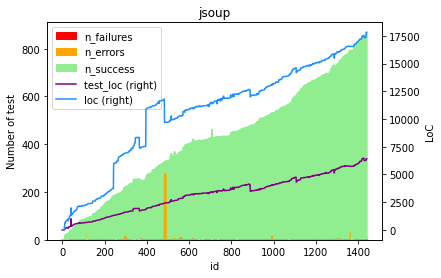
\includegraphics[width=\textwidth]{pages/02-Testability/images/projects/jsoup.png}
        \label{fig:jsoup}
    \end{minipage}%
    \begin{minipage}{.5\linewidth}
        \centering
        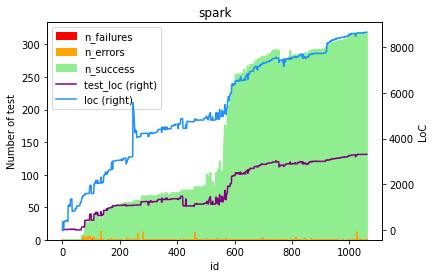
\includegraphics[width=\textwidth]{pages/02-Testability/images/projects/spark.png}
        \label{fig:spark}
    \end{minipage}
    \begin{minipage}{.5\linewidth}
        \centering
        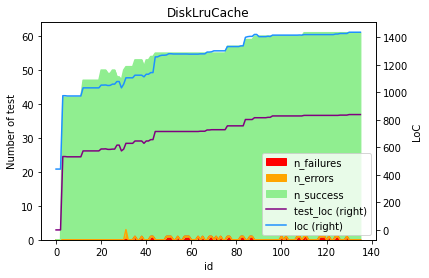
\includegraphics[width=\textwidth]{pages/02-Testability/images/projects/disklrucache.png}
        \label{fig:disklrucache}
    \end{minipage}%
    \begin{minipage}{.5\linewidth}
        \centering
        \begin{tabular}{|r|r|r|}
        \hline
        \textbf{Project} & \textbf{TestBuildability} & \textbf{FullyTestability} \\ \hline
        jsoup            & 97.29\%                      & 93.55\%                      \\ \hline
        spark            & 92.84\%                      & 86.72\%                      \\ \hline
        DiskLruCache     & 97.79\%                      & 70.58\%                      \\ \hline
        \end{tabular}
        \vspace*{0.5cm}
        \captionof{table}{Metrics of set of projects 1: JSoup, Spark and DiskLRUCache}
        \label{table:projects-1}
    \end{minipage} 
\end{figure}

% \begin{figure}[h!]
%     \centering
%     \begin{subfigure}[b]{0.45\textwidth}
%         \centering
%         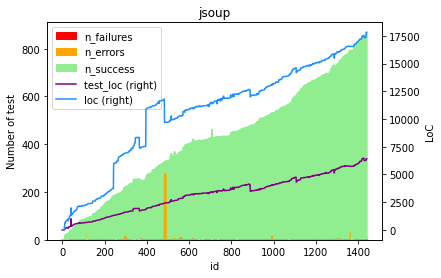
\includegraphics[width=\textwidth]{pages/02-Testability/images/projects/jsoup.png}
%         \label{fig:jsoup}
%     \end{subfigure}
%     \hfill
%     \begin{subfigure}[b]{0.45\textwidth}
%         \centering
%         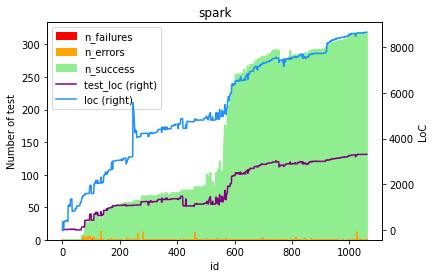
\includegraphics[width=\textwidth]{pages/02-Testability/images/projects/spark.png}
%         \label{fig:spark}
%     \end{subfigure}
%     \hfill
%     \begin{subfigure}[b]{0.45\textwidth}
%         \centering
%         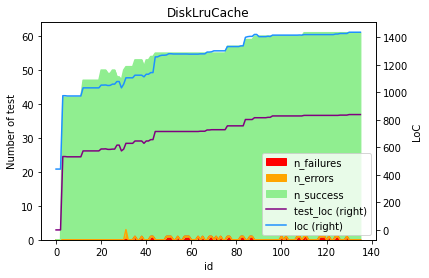
\includegraphics[width=\textwidth]{pages/02-Testability/images/projects/disklrucache.png}
%         \label{fig:disklrucache}
%     \end{subfigure}
%        \caption{Set of projects 1: DiskLRUCache, Spark and JSoup}
%        \label{fig:projects-1}
% \end{figure}

% \begin{table}[h!]
%     \centering
%     \begin{tabular}{|r|r|r|}
%     \hline
%     \textbf{Project} & \textbf{TestBuildability} & \textbf{FullyTestability} \\ \hline
%     jsoup            & 99.50\%                     & 93.55\%                      \\ \hline
%     spark            & 93.81\%                      & 86.72\%                      \\ \hline
%     DiskLruCache     & 97.79\%                      & 70.58\%                      \\ \hline
%     \end{tabular}
%     \caption{Metrics of set of projects 1: JSoup, Spark and DiskLRUCache}
%     \label{table:projects-1}
% \end{table}

%%%%%%%%%%%%%%%%%%%%%%%%%%%%%%%%%%%%%%%%%%%%%%%%%%%%%%%%%%%%%%%%%%%%%
%                           SECOND SET                              %
%%%%%%%%%%%%%%%%%%%%%%%%%%%%%%%%%%%%%%%%%%%%%%%%%%%%%%%%%%%%%%%%%%%%%

The second set of project that we are going to study (Figure~\ref{fig:projects-2}) have been selected as a representative set of projects that, taking a look at their visual representation, it seems that it is possible to run the tests in the past in almost all their history, although in some of them we find multiple commits where failures or bugs are located.
However, if we look again at the FullyTestability values (Table~\ref{table:projects-2}), we find that their values are surprisingly low. 
For example, the \textit{Checkstyle} project, despite the fact that a portion of its commits at the beginning of the project are not buildable, the figure seems to indicate that almost all of its tests pass. 
Its low FullyTestability value is due to a few tests fail along the project history.
% \michel{He vuelto a mirar muy en detalle, parece que al re-ejecutarlo han cambiado un poco los resultados. En un párrafo no puedo comentarte exacatemente lo que he encontrado. Tengo que enseñarte las tablas y comentarte. Rápidamente puedo decir que en este proyecto solo pasan los test en el 0.01\% de los commtis (81). En la mayoria de commits, un porcentaje muy bajo de test fallan. En un commit en concreto fallan 17 test, pero en los demás es menos de 10 (con +1000 test). Hay test que fallan en todos los commits, pero no son muchos (17 test únicos). Hay un par de test más que fallan en muy pocos commits. Para ver los logs de porqué fallan esos test tengo que bajarme los resultados de Minio y descomprimirlos, por lo que me gustaría comentarlo antes}
The other two projects are similar, in the case of \textit{HikariCP} the failures are more visible in the graph despite having the highest FullyTestability value of this set.

\begin{figure}[!htb]
    \caption{Set of projects 2: Fastjson, Checkstyle and HikariCP}
    \label{fig:projects-2}
    \begin{minipage}{.5\linewidth}
        \centering
        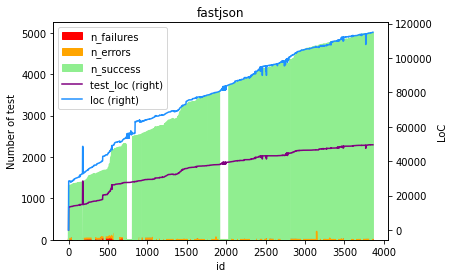
\includegraphics[width=\textwidth]{pages/02-Testability/images/projects/fastjson.png}
        \label{fig:fastjson}
    \end{minipage}%
    \begin{minipage}{.5\linewidth}
        \centering
        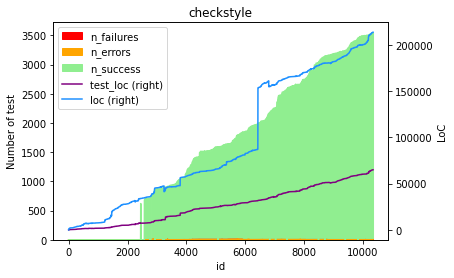
\includegraphics[width=\textwidth]{pages/02-Testability/images/projects/checkstyle.png}
        \label{fig:checkstyle}
    \end{minipage}
    \begin{minipage}{.5\linewidth}
        \centering
        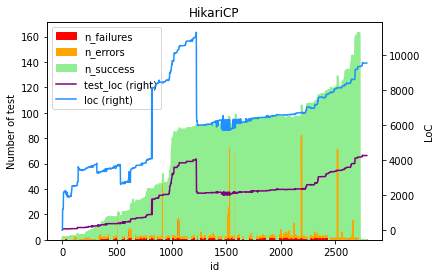
\includegraphics[width=\textwidth]{pages/02-Testability/images/projects/hikari.png}
        \label{fig:hikari}
    \end{minipage}%
    \begin{minipage}{.5\linewidth}
        \centering
        \begin{tabular}{|r|r|r|}
        \hline
        \textbf{Project} & \textbf{TestBuildability} & \textbf{FullyTestability} \\ \hline
        HikariCP         & 95.22\%                      & 16.92\%                      \\ \hline
        Checkstyle       & 74.35\%                      & 0.78\%                      \\ \hline
        Fastjson         & 88.35\%                      & 0.00\%                      \\ \hline
        \end{tabular}
        \vspace*{0.5cm}
        \captionof{table}{Metrics of set of projects 2: Fastjson, Checkstyle and HikariCP}
        \label{table:projects-2}
    \end{minipage} 
\end{figure}

% \begin{figure}[h!]
%     \centering
%     \begin{subfigure}[b]{0.45\textwidth}
%         \centering
%         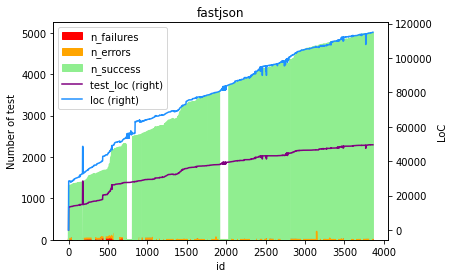
\includegraphics[width=\textwidth]{pages/02-Testability/images/projects/fastjson.png}
%         \label{fig:fastjson}
%     \end{subfigure}
%     \hfill
%     \begin{subfigure}[b]{0.45\textwidth}
%         \centering
%         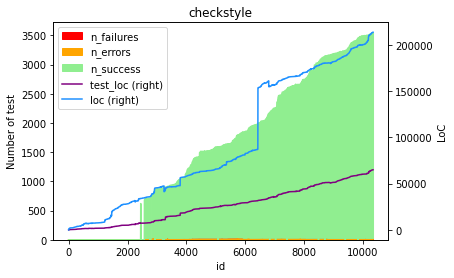
\includegraphics[width=\textwidth]{pages/02-Testability/images/projects/checkstyle.png}
%         \label{fig:checkstyle}
%     \end{subfigure}
%     \hfill
%     \begin{subfigure}[b]{0.45\textwidth}
%         \centering
%         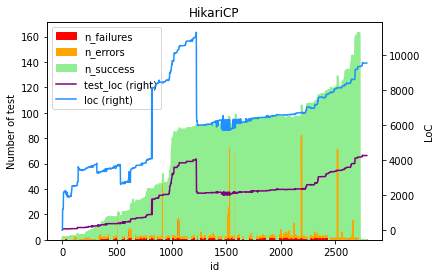
\includegraphics[width=\textwidth]{pages/02-Testability/images/projects/hikari.png}
%         \label{fig:hikari}
%     \end{subfigure}
%        \caption{Set of projects 2: Fastjson, Checkstyle and HikariCP}
%        \label{fig:projects-2}
% \end{figure}

% \begin{table}[h!]
%     \centering
%     \begin{tabular}{|r|r|r|}
%     \hline
%     \textbf{Project} & \textbf{TestBuildability} & \textbf{FullyTestability} \\ \hline
%     Fastjson         & 93.73\%                      & 0.00\%                      \\ \hline
%     Checkstyle       & 95.66\%                      & 0.01\%                      \\ \hline
%     HikariCP         & 99.17\%                      & 16.92\%                      \\ \hline
%     \end{tabular}
%     \caption{Metrics of set of projects 1: Fastjson, Checkstyle and HikariCP}
%     \label{table:projects-2}
% \end{table}

Considering the above-mentioned, FullyTestability is a very restrictive metric, as soon as a project test, present in most commits, does not work, it drastically reduces the value of the metric. 
We can consider that we are missing information about the real testability of the project.
From the point of view of a practitioner or a researcher who needs to add a change to a past version and has to evaluate if the tests allow him to be sure not to introduce any regression in the code, knowing that in a commit 99.99\% of the tests pass (as happened in the case of the \textit{Checkstyle} project, where there are commits with 3506 tests but only 1 fails) may be enough.

Following this discussion, we propose a new and less restrictive way of measuring testability, which allows us to capture the information in a non-binary way. 
Instead of using a binary value (a commit is either FullyTestable or not) we will use a ratio. 
Hence, a commit has a \textbf{TestableRate}, defined as the ratio of success tests with respect to the total number of tests intended to run for that commit.
For a project, we would obtain the \textbf{TestabilityRate} as the mean of the TestableRate value of all commits in the history.

Table~\ref{table:projects-2-with-testability-rate} shows the TestabilityRate results for the second set of projects.
This new metric reflects a higher testability value for this set of projects, which is in line with the reality of the tests executed.

\begin{table}[h!]
    \centering
    \begin{tabular}{|r|r|r|r|}
        \hline
        \textbf{Project} & \textbf{TestBuildability} & \textbf{FullyTestability} & \textbf{TestabilityRate} \\ \hline
        HikariCP         & 95.22\%                      & 16.92\%                      & 88.76\%                     \\ \hline
        checkstyle       & 74.35\%                      & 0.78\%                       & 74.22\%                     \\ \hline
        fastjson         & 88.35\%                      & 0.00\%                       & 87.80\%                     \\ \hline
        \end{tabular}
    \caption{Metrics of set of projects 1: Fastjson, Checkstyle and HikariCP (including the new TestabilityRate metric)}
    \label{table:projects-2-with-testability-rate}
\end{table}

%%%%%%%%%%%%%%%%%%%%%%%%%%%%%%%%%%%%%%%%%%%%%%%%%%%%%%%%%%%%%%%%%%%%%
%                            THIRD SET                              %
%%%%%%%%%%%%%%%%%%%%%%%%%%%%%%%%%%%%%%%%%%%%%%%%%%%%%%%%%%%%%%%%%%%%%

The third set of projects is shown in Figure~\ref{fig:projects-3}. 
In this case, we have chosen projects that appear to be very testable but only in a part of their history (due to problems in building the source code or test code).
Table~\ref{table:projects-3} shows the testability values for these projects. 

\begin{figure}[!htb]
    \caption{Set of projects 3: Zxing, Okio and Closure}
    \label{fig:projects-3}
    \begin{minipage}{.5\linewidth}
        \centering
        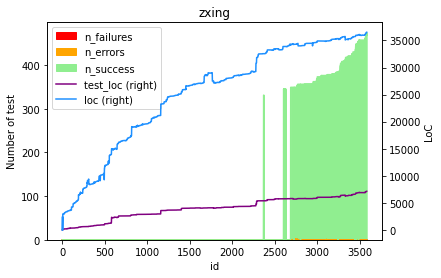
\includegraphics[width=\textwidth]{pages/02-Testability/images/projects/zxing.png}
        \label{fig:zxing}
    \end{minipage}%
    \begin{minipage}{.5\linewidth}
        \centering
        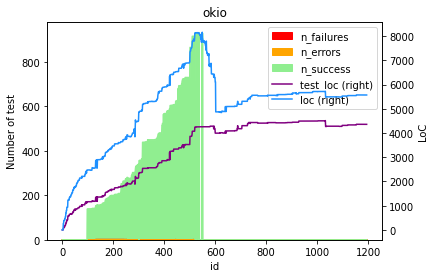
\includegraphics[width=\textwidth]{pages/02-Testability/images/projects/okio.png}
        \label{fig:okio}
    \end{minipage}
    \begin{minipage}{.5\linewidth}
        \centering
        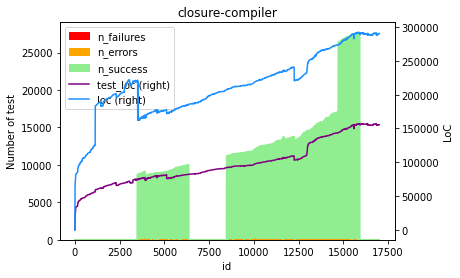
\includegraphics[width=\textwidth]{pages/02-Testability/images/projects/closure.png}
        \label{fig:closure-compiler}
    \end{minipage}%
    \begin{minipage}{.5\linewidth}
        \centering
        \begin{tabular}{|r|r|r|r|}
            \hline
            \textbf{Project} & \multicolumn{1}{c|}{\textbf{\begin{tabular}[c]{@{}c@{}}Test \\ Buildability\end{tabular}}} & \multicolumn{1}{c|}{\textbf{\begin{tabular}[c]{@{}c@{}}Fully\\ Testability\end{tabular}}} & \multicolumn{1}{c|}{\textbf{\begin{tabular}[c]{@{}c@{}}Testability\\ Rate\end{tabular}}} \\ \hline
            okio             & 36.06\%                      & 26.27\%                       & 36.01\%                     \\ \hline
            closure          & 59.84\%                      & 55.81\%                       & 59.84\%                     \\ \hline
            zxing            & 25.39\%                      & 24.80\%                       & 25.38\%                     \\ \hline
        \end{tabular}
        \vspace*{0.5cm}
        \captionof{table}{Metrics of set of projects 3: Zxing, Okio and Closure}
        \label{table:projects-3}
    \end{minipage} 
\end{figure}

These projects are characterized by a low TestBuildability. 
The TestBuildability metric is greatly affected by SourceBuildability; if the code does not compile, the tests cannot be compiled. 
The reasons why source code cannot be compiled have been studied in previous work~\cite{tufano2017there,Sulir:2016:QSJ:3001878.3001882}, mainly because of the impossibility to reproduce the context and retrieve the dependencies of a particular commit. 
For the okio, closure and zxing projects, the SourceBuildability values are 36.65, 60.18 and 25.47 respectively, very close to TestBuildability values.
\michel{No estoy muy seguro de si deberia meter estos datos en la tabla \ref{table:projects-3}}
So, we can state that in these projects, if the source code compiles, in most cases the test code compiles as well. 
We can reflect this in a new metric: TestBuildability\textsubscript{S}, the ratio of test-buildable commits with respect to the source-buildable commits.
The TestBuildability metric, when calculated considering all commits in the project history, is renamed to TestBuildability\textsubscript{A}.
Table~\ref{table:projects-3-B} shows the values of these two variants of TestBuildability, in addition to the SourceBuildability values mentioned above.

\begin{table}[h!]
    \centering
    \begin{tabular}{|r|r|r|r|r|r|}
    \hline
    \multicolumn{1}{|c|}{\textbf{Project}} & \multicolumn{1}{c|}{\textbf{\begin{tabular}[c]{@{}c@{}}Source \\ Buildability\end{tabular}}} & \multicolumn{1}{c|}{\textbf{\begin{tabular}[c]{@{}c@{}}Test \\ Buildability\textsubscript{A}\end{tabular}}} & \multicolumn{1}{c|}{\textbf{\begin{tabular}[c]{@{}c@{}}Test \\ Buildability\textsubscript{S}\end{tabular}}} & \multicolumn{1}{c|}{\textbf{\begin{tabular}[c]{@{}c@{}}Fully\\ Testability\end{tabular}}} & \multicolumn{1}{c|}{\textbf{\begin{tabular}[c]{@{}c@{}}Testability\\ Rate\end{tabular}}} \\ \hline
    okio                                   & 36.65\%                                                                                        & 36.07\%                                                                                         & 98.40\%                                                                                         & 26.28\%                                                                                     & 36.02\%                                         \\ \hline
    closure-compiler                       & 60.18\%                                                                                        & 59.84\%                                                                                         & 99.43\%                                                                                         & 55.82\%                                                                                     & 59.84\%                                         \\ \hline
    zxing                                  & 25.47\%                                                                                        & 25.39\%                                                                                         & 99.67\%                                                                                         & 24.80\%                                                                                     & 25.39\%                                         \\ \hline
    \end{tabular}
    \captionof{table}{Extended metrics of set of projects 3: Zxing, Okio and Closure}
    \label{table:projects-3-B}
\end{table}

Following the idea of focusing on those commits where we can build the test code, we should consider that it is possible that the commits that do not compile, never did and therefore their testability information is not useful to us.
% Once again we find that the testability metrics do not provide all the information. 
% When we cannot build source code or test code, we lose testability information. 
For projects such as those in set 3, the testability of the commits where we can build the tests gives us valuable information that neither the FullyTestability nor the TestabilityRate capture, as both metrics are calculated from all commits in the history of the project.

To capture the testability of Test Buildable commits we define the following metrics:
\begin{itemize}
    \item \textbf{TestabilityRate\textsubscript{T}}: mean of \textit{testable rate} for \textit{test-buildable commits} in the project.
    \item \textbf{FullyTestability\textsubscript{T}}: ratio of \textit{fully testable commits} with respect to the number of \textit{test-buildable commits} of the project.
\end{itemize}
The FullyTestability and TestabilityRate metrics, when calculated considering all the commits in the history, are renamed FullyTestability\textsubscript{A} and TestabilityRate\textsubscript{A}.

In Table~\ref{table:projects-3-with-flavor-testability-rate} we include the new metrics defined for the third set of projects. 
We note that for all 3 projects, the new metrics more closely capture the testability of the commits we can build.
The FullyTestability\textsubscript{T} shows us that for those commits where we can build the tests, a high percentage can run all their tests with a success result. For this same set of commits, the TestabilityRate\textsubscript{T} shows us values close to 100\%; almost all of the tests in these commits offer a success result.

\begin{table*}[h!]
    \centering
    \begin{tabular}{|r|r|r|r|r|r|r|r|}
        \hline
        \multicolumn{1}{|c|}{\textbf{Project}} & \multicolumn{1}{c|}{\textbf{\begin{tabular}[c]{@{}c@{}}Source \\ Buildability\end{tabular}}} & \multicolumn{1}{c|}{\textbf{\begin{tabular}[c]{@{}c@{}}Test \\ Buildability\textsubscript{A}\end{tabular}}} & \multicolumn{1}{c|}{\textbf{\begin{tabular}[c]{@{}c@{}}Test \\ Buildability\textsubscript{S}\end{tabular}}} & \multicolumn{1}{c|}{\textbf{\begin{tabular}[c]{@{}c@{}}Fully\\ Testability\textsubscript{A}\end{tabular}}} & \multicolumn{1}{c|}{\textbf{\begin{tabular}[c]{@{}c@{}}Fully\\ Testability\textsubscript{T}\end{tabular}}} & \multicolumn{1}{c|}{\textbf{\begin{tabular}[c]{@{}c@{}}Testability\\ Rate\textsubscript{A}\end{tabular}}} & \multicolumn{1}{c|}{\textbf{\begin{tabular}[c]{@{}c@{}}Testability\\ Rate\textsubscript{T}\end{tabular}}} \\ \hline
        okio                                   & 36.65\%                                                                                        & 36.07\%                                                                                       & 98.40\%                                                                                       & 26.28\%                                                                                      & 72.85\%                                                                                      & 36.02\%                                                                                     & 99.86\%                                                                                     \\ \hline
        closure                                & 60.18\%                                                                                        & 59.84\%                                                                                       & 99.43\%                                                                                       & 55.82\%                                                                                      & 93.27\%                                                                                      & 59.84\%                                                                                     & 99.99\%                                                                                     \\ \hline
        zxing                                  & 25.47\%                                                                                        & 25.39\%                                                                                       & 99.67\%                                                                                       & 24.80\%                                                                                      & 97.69\%                                                                                      & 25.39\%                                                                                     & 99.99\%                                                                                    \\ \hline
    \end{tabular}
    \caption{Extended metrics of set of projects 3: Zxing, Okio and Closure (including the new TestabilityRate\textsubscript{T} and FullyTestability\textsubscript{T} metrics)}
    \label{table:projects-3-with-flavor-testability-rate}
\end{table*}

\patxi{Podría ser interesante incluir también o analizar los del conjunto 1, para dar una idea de la robustez de esta métrica: ¿sigue manteniéndose alta en el primer conjunto de proyectos y refleja por tanto lo que queremos?}
\michel{Temo sobrecargar esta sección de tablas, a continuación te dejo esa tabla que comentas (sin formatear). Mi impresión es que las métricas son esperables teniendo en cuenta los razonamientos que hemos hecho, no aportan nada nuevo.}

\def \RQIII{How many tests of a snapshot can be run with a `success' result?}

This case study helped us to define metrics that better describe a project's stability. These new metrics lead to a new research question: 

\textbf{RQ\textsubscript{3}}: ``\RQIII''
\michel{Habría quedar una vuelta a la pregunta}